% This template has been adapted from https://github.com/jgm/pandoc-templates
% that comes attached with the following copyright notice.
%
% Copyright (c) 2014--2017, John MacFarlane
%
% All rights reserved.
%
% Redistribution and use in source and binary forms, with or without
% modification, are permitted provided that the following conditions are met:
%
% * Redistributions of source code must retain the above copyright notice,
%   this list of conditions and the following disclaimer.
% * Redistributions in binary form must reproduce the above copyright notice,
%   this list of conditions and the following disclaimer in the documentation
%   and/or other materials provided with the distribution.
% * Neither the name of John MacFarlane nor the names of other contributors may
%   be used to endorse or promote products derived from this software without
%   specific prior written permission.
%
% THIS SOFTWARE IS PROVIDED BY THE COPYRIGHT HOLDERS AND CONTRIBUTORS "AS IS"
% AND ANY EXPRESS OR IMPLIED WARRANTIES, INCLUDING, BUT NOT LIMITED TO, THE
% IMPLIED WARRANTIES OF MERCHANTABILITY AND FITNESS FOR A PARTICULAR PURPOSE
% ARE DISCLAIMED. IN NO EVENT SHALL THE COPYRIGHT OWNER OR CONTRIBUTORS BE
% LIABLE FOR ANY DIRECT, INDIRECT, INCIDENTAL, SPECIAL, EXEMPLARY, OR
% CONSEQUENTIAL DAMAGES (INCLUDING, BUT NOT LIMITED TO, PROCUREMENT OF
% SUBSTITUTE GOODS OR SERVICES; LOSS OF USE, DATA, OR PROFITS; OR BUSINESS
% INTERRUPTION) HOWEVER CAUSED AND ON ANY THEORY OF LIABILITY, WHETHER IN
% CONTRACT, STRICT LIABILITY, OR TORT (INCLUDING NEGLIGENCE OR OTHERWISE)
% ARISING IN ANY WAY OUT OF THE USE OF THIS SOFTWARE, EVEN IF ADVISED OF THE
% POSSIBILITY OF SUCH DAMAGE.

\documentclass[
  headsepline=true,headings=standardclasses%
]{scrartcl}

\usepackage{ifxetex,ifluatex}


\ifnum 0\ifxetex 1\fi\ifluatex 1\fi=0 % if pdftex

\usepackage[T1]{fontenc}
\usepackage[utf8]{inputenc}

\usepackage{amsthm}
% libertine + biolinum
\usepackage[lining]{libertine}
\usepackage{textcomp}
\usepackage[varqu,varl]{inconsolata}
\usepackage[libertine,libaltvw,liby,vvarbb]{newtxmath}
\usepackage[scr=rsfso]{mathalfa}
\usepackage{bm}
\useosf


\else % if luatex or xelatex
\usepackage{lmodern}
\usepackage{amssymb,amsthm}

\usepackage{unicode-math}
\defaultfontfeatures{Ligatures=TeX,Scale=MatchLowercase}
\fi

% use upquote if available, for straight quotes in verbatim environments
\IfFileExists{upquote.sty}{\usepackage{upquote}}{}

% use microtype if available
\IfFileExists{microtype.sty}{%
\usepackage{microtype}
\UseMicrotypeSet[protrusion]{basicmath} % disable protrusion for tt fonts
}{}

\usepackage{hyperref}
\PassOptionsToPackage{usenames,dvipsnames}{color} % color is loaded by hyperref
\hypersetup{
  unicode=true,
  pdftitle={eulerr: Area-Proportional Euler Diagrams with Ellipses},
  colorlinks=true,
  linkcolor=Maroon,
  citecolor=Blue,
  urlcolor=Blue,
  breaklinks=true
}
\urlstyle{same}  % don't use monospace font for urls

% Language options (babel/polyglossia)

% Captions
\usepackage[labelfont=bf,labelsep=period,font=small]{caption}

% Floats
\usepackage{floatrow}
\usepackage{stfloats}
\fnbelowfloat % puts footnotes below the bottom floats
\floatsetup[table]{capposition=top}




\usepackage{color}
\usepackage{fancyvrb}
\newcommand{\VerbBar}{|}
\newcommand{\VERB}{\Verb[commandchars=\\\{\}]}
\DefineVerbatimEnvironment{Highlighting}{Verbatim}{commandchars=\\\{\}}
% Add ',fontsize=\small' for more characters per line
\usepackage{framed}
\definecolor{shadecolor}{RGB}{248,248,248}
\newenvironment{Shaded}{\begin{snugshade}}{\end{snugshade}}
\newcommand{\KeywordTok}[1]{\textcolor[rgb]{0.13,0.29,0.53}{\textbf{#1}}}
\newcommand{\DataTypeTok}[1]{\textcolor[rgb]{0.13,0.29,0.53}{#1}}
\newcommand{\DecValTok}[1]{\textcolor[rgb]{0.00,0.00,0.81}{#1}}
\newcommand{\BaseNTok}[1]{\textcolor[rgb]{0.00,0.00,0.81}{#1}}
\newcommand{\FloatTok}[1]{\textcolor[rgb]{0.00,0.00,0.81}{#1}}
\newcommand{\ConstantTok}[1]{\textcolor[rgb]{0.00,0.00,0.00}{#1}}
\newcommand{\CharTok}[1]{\textcolor[rgb]{0.31,0.60,0.02}{#1}}
\newcommand{\SpecialCharTok}[1]{\textcolor[rgb]{0.00,0.00,0.00}{#1}}
\newcommand{\StringTok}[1]{\textcolor[rgb]{0.31,0.60,0.02}{#1}}
\newcommand{\VerbatimStringTok}[1]{\textcolor[rgb]{0.31,0.60,0.02}{#1}}
\newcommand{\SpecialStringTok}[1]{\textcolor[rgb]{0.31,0.60,0.02}{#1}}
\newcommand{\ImportTok}[1]{#1}
\newcommand{\CommentTok}[1]{\textcolor[rgb]{0.56,0.35,0.01}{\textit{#1}}}
\newcommand{\DocumentationTok}[1]{\textcolor[rgb]{0.56,0.35,0.01}{\textbf{\textit{#1}}}}
\newcommand{\AnnotationTok}[1]{\textcolor[rgb]{0.56,0.35,0.01}{\textbf{\textit{#1}}}}
\newcommand{\CommentVarTok}[1]{\textcolor[rgb]{0.56,0.35,0.01}{\textbf{\textit{#1}}}}
\newcommand{\OtherTok}[1]{\textcolor[rgb]{0.56,0.35,0.01}{#1}}
\newcommand{\FunctionTok}[1]{\textcolor[rgb]{0.00,0.00,0.00}{#1}}
\newcommand{\VariableTok}[1]{\textcolor[rgb]{0.00,0.00,0.00}{#1}}
\newcommand{\ControlFlowTok}[1]{\textcolor[rgb]{0.13,0.29,0.53}{\textbf{#1}}}
\newcommand{\OperatorTok}[1]{\textcolor[rgb]{0.81,0.36,0.00}{\textbf{#1}}}
\newcommand{\BuiltInTok}[1]{#1}
\newcommand{\ExtensionTok}[1]{#1}
\newcommand{\PreprocessorTok}[1]{\textcolor[rgb]{0.56,0.35,0.01}{\textit{#1}}}
\newcommand{\AttributeTok}[1]{\textcolor[rgb]{0.77,0.63,0.00}{#1}}
\newcommand{\RegionMarkerTok}[1]{#1}
\newcommand{\InformationTok}[1]{\textcolor[rgb]{0.56,0.35,0.01}{\textbf{\textit{#1}}}}
\newcommand{\WarningTok}[1]{\textcolor[rgb]{0.56,0.35,0.01}{\textbf{\textit{#1}}}}
\newcommand{\AlertTok}[1]{\textcolor[rgb]{0.94,0.16,0.16}{#1}}
\newcommand{\ErrorTok}[1]{\textcolor[rgb]{0.64,0.00,0.00}{\textbf{#1}}}
\newcommand{\NormalTok}[1]{#1}


\usepackage{longtable,booktabs}

\usepackage{graphicx,grffile}
\makeatletter
\def\maxwidth{\ifdim\Gin@nat@width>\linewidth\linewidth\else\Gin@nat@width\fi}
\def\maxheight{\ifdim\Gin@nat@height>\textheight\textheight\else\Gin@nat@height\fi}
\makeatother
% Scale images if necessary, so that they will not overflow the page
% margins by default, and it is still possible to overwrite the defaults
% using explicit options in \includegraphics[width, height, ...]{}
\setkeys{Gin}{width=\maxwidth,height=\maxheight,keepaspectratio}



\providecommand{\tightlist}{\setlength{\itemsep}{0pt}\setlength{\parskip}{0pt}}

% Redefines (sub)paragraphs to behave more like sections
\ifx\paragraph\undefined\else
\let\oldparagraph\paragraph
\renewcommand{\paragraph}[1]{\oldparagraph{#1}\mbox{}}
\fi
\ifx\subparagraph\undefined\else
\let\oldsubparagraph\subparagraph
\renewcommand{\subparagraph}[1]{\oldsubparagraph{#1}\mbox{}}
\fi


% set default figure placement to htbp
\makeatletter
\def\fps@figure{htbp}
\makeatother

% Use protect on footnotes to avoid problems with footnotes in titles
\let\rmarkdownfootnote\footnote%
\def\footnote{\protect\rmarkdownfootnote}

\title{eulerr: Area-Proportional Euler Diagrams with Ellipses}

\subtitle{Bachelor Thesis}

% Subfigs
\usepackage{subfig}

% Authors
\usepackage[noblocks]{authblk}
\renewcommand\Affilfont{\itshape\small}
\renewcommand\Authfont{}

\author[]{Johan Larsson}
\author[]{Peter Gustafsson}

\affil[]{Lund University}

\date{2017-08-15}

% Headers and footers
\usepackage{scrlayer-scrpage}
\pagestyle{scrheadings}

\automark[subsection]{section}
\clearmainofpairofpagestyles
\lohead[]{\headmark}
\cfoot[\pagemark]{\pagemark}

\rohead[]{eulerr}


% KOMA font options
\setkomafont{descriptionlabel}{\normalfont\scshape\bfseries}


% KOMA options


\usepackage{amsthm}
\newtheorem{theorem}{Theorem}[section]
\newtheorem{lemma}{Lemma}[section]
\theoremstyle{definition}
\newtheorem{definition}{Definition}[section]
\newtheorem{corollary}{Corollary}[section]
\newtheorem{proposition}{Proposition}[section]
\theoremstyle{definition}
\newtheorem{example}{Example}[section]
\theoremstyle{remark}
\newtheorem*{remark}{Remark}
\begin{document}
\maketitle



\hypersetup{linkcolor=black}
\setcounter{tocdepth}{2}
\tableofcontents



\section{Introduction}\label{introduction}

Relationships between groups and sets are the focus in many scientific
disciplines. In biomedicine, for instance, the overlap between sets of
genes may be of interest. In epidemiology, the interactions between
diseases are frequently studied. Likewise, the social sciences are often
involved in studying demographics where the commonalities between
various groups are scrutinized.

Visualizations of such relationships are central to understanding them.
The commonest visualization is Venn diagrams. Venn diagrams are a subset
of Euler diagrams, which were originally proposed by Leonard Euler
(1707--1783) {[}1{]}. Whereas Venn diagrams require that all
2\textsuperscript{n} possible intersection are present -- even if they
are empty -- Euler diagrams stipulate no such requirement.

Euler diagrams can be area-proportional, which is the case for non-Venn
diagrams. Area-proportional diagrams are most easily understood as their
interpretations do not depend on any numbers. This paper will henceforth
be concerned only with such designs and the term \emph{Euler diagram}
will be considered to refer to area-proportional diagrams.

Euler diagrams may be fashioned with any conceivable closed shape.\\
Solutions have been developed for triangles {[}2{]}, rectangles {[}2{]},
ellipses {[}3{]}, smooth curves, polygons {[}2{]}, and circles
{[}2,4,5{]}. The latter is most common, and appears to be preferred for
optimal readability {[}citation{]}. Yet circles do not always lend
themselves to accurate representations. Consider, for instance the
combination \[
\begin{gathered}
A = B = C = 2,\\
A \cap B = A \cap C = B \cap C = 1, \text{ and}\\
A \cap B \cap C = 0.
\end{gathered}
\] There is no way to visualize this relationship perfectly with circles
(Figure \ref{fig:impossible3}).

\begin{Shaded}
\begin{Highlighting}[]
\KeywordTok{library}\NormalTok{(eulerr)}
\KeywordTok{library}\NormalTok{(latticeExtra)}
\NormalTok{p1 <-}\StringTok{ }\KeywordTok{plot}\NormalTok{(}\KeywordTok{euler}\NormalTok{(}\KeywordTok{c}\NormalTok{(}\DataTypeTok{A =} \DecValTok{2}\NormalTok{, }\DataTypeTok{B =} \DecValTok{2}\NormalTok{, }\DataTypeTok{C =} \DecValTok{2}\NormalTok{, }\StringTok{"A&B"}\NormalTok{ =}\StringTok{ }\DecValTok{1}\NormalTok{, }\StringTok{"A&C"}\NormalTok{ =}\StringTok{ }\DecValTok{1}\NormalTok{, }\StringTok{"B&C"}\NormalTok{ =}\StringTok{ }\DecValTok{1}\NormalTok{)))}
\NormalTok{p2 <-}\StringTok{ }\KeywordTok{plot}\NormalTok{(}\KeywordTok{euler}\NormalTok{(}\KeywordTok{c}\NormalTok{(}\DataTypeTok{A =} \DecValTok{2}\NormalTok{, }\DataTypeTok{B =} \DecValTok{2}\NormalTok{, }\DataTypeTok{C =} \DecValTok{2}\NormalTok{, }\StringTok{"A&B"}\NormalTok{ =}\StringTok{ }\DecValTok{1}\NormalTok{, }\StringTok{"A&C"}\NormalTok{ =}\StringTok{ }\DecValTok{1}\NormalTok{, }\StringTok{"B&C"}\NormalTok{ =}\StringTok{ }\DecValTok{1}\NormalTok{),}
                 \DataTypeTok{shape =} \StringTok{"ellipse"}\NormalTok{))}
\KeywordTok{c}\NormalTok{(p1, p2)}
\end{Highlighting}
\end{Shaded}

\begin{figure}
\centering
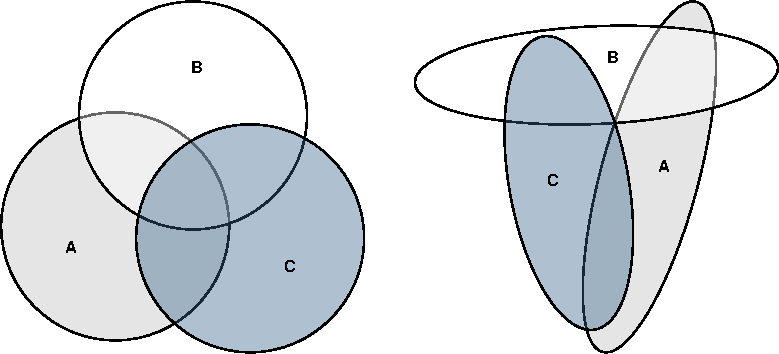
\includegraphics{thesis_files/figure-latex/impossible3-1.pdf}
\caption{\label{fig:impossible3}A set relationship depicted with circles and
ellipses.}
\end{figure}

For four intersecting sets, circular Euler diagrams are in fact
impossible since they require \(2^4=16\) regions but four intersecting
circles yield at most 14 unique intersections. This is not, however, the
case with ellipses being that they may intersect in up to 4, rather than
2, points. And because ellipses can be rotated, they can succeed where
circles fail (Figure \ref{fig:impossible3}).

Elliptical Euler diagrams have been successfully implemented in the
\textbf{eulerAPE} software {[}3{]} but only for three sets that all need
to intersect. It is implemented in

\section{Method}\label{method}

\subsection{Areas of overlapping
ellipses}\label{areas-of-overlapping-ellipses}

\subsection{Visualization}\label{visualization}

\section{Results}\label{results}

\subsection{Consistency}\label{consistency}

\subsection{Accuracy}\label{accuracy}

\subsection{Performance}\label{performance}

\section{Discussion}\label{discussion}

\textbf{eulerr} relies on an extensive machinery to turn user input into
a pretty Euler diagram. Little, or in fact none, of this requires any
tinkering from the user. To make that happen, however, \textbf{eulerr}
needs to make several well-formed decisions about the design of the
diagram on behalf of the user, which is not a trivial task.

This document outlines the implementation of \textbf{eulerr} from input
to output. It is designed to an up-to-date paper on the innards of the
program and is therefore likely to evolve as time goes on.

\section{Input}\label{input}

The main function of \textbf{eulerr} is \texttt{euler()}. To start with,
we need input in the form of

\begin{itemize}
\tightlist
\item
  a named numeric vector, such as
  \texttt{c(A\ =\ 10,\ B\ =\ 5,\ "A\&B"\ =\ 3)}, where ampersands define
  disjoint set combinations or unions, depending on the argument
  \texttt{input},
\item
  a \texttt{data.frame} or \texttt{matrix} of logicals or binary indices
  where each row denotes the set relationships of
\item
  either a single observation
\end{itemize}

\begin{Shaded}
\begin{Highlighting}[]
\KeywordTok{matrix}\NormalTok{(}\KeywordTok{sample}\NormalTok{(}\KeywordTok{c}\NormalTok{(}\OtherTok{TRUE}\NormalTok{, }\OtherTok{FALSE}\NormalTok{), }\DecValTok{12}\NormalTok{, }\DataTypeTok{replace =} \OtherTok{TRUE}\NormalTok{),}
       \DataTypeTok{ncol =} \DecValTok{3}\NormalTok{,}
       \DataTypeTok{dimnames =} \KeywordTok{list}\NormalTok{(}\OtherTok{NULL}\NormalTok{, }\KeywordTok{c}\NormalTok{(}\StringTok{"A"}\NormalTok{, }\StringTok{"B"}\NormalTok{, }\StringTok{"C"}\NormalTok{)))}
\end{Highlighting}
\end{Shaded}

\begin{verbatim}
##          A     B     C
## [1,] FALSE FALSE FALSE
## [2,]  TRUE FALSE  TRUE
## [3,] FALSE  TRUE FALSE
## [4,]  TRUE FALSE  TRUE
\end{verbatim}

\begin{itemize}
\tightlist
\item
  or of a unique set combination if a numeric vector is supplied to the
  argument \texttt{weights},
\end{itemize}

\begin{Shaded}
\begin{Highlighting}[]
\KeywordTok{matrix}\NormalTok{(}\KeywordTok{c}\NormalTok{(}\OtherTok{TRUE}\NormalTok{, }\OtherTok{FALSE}\NormalTok{, }\OtherTok{FALSE}\NormalTok{,}
         \OtherTok{TRUE}\NormalTok{, }\OtherTok{TRUE}\NormalTok{, }\OtherTok{FALSE}\NormalTok{,}
         \OtherTok{FALSE}\NormalTok{, }\OtherTok{FALSE}\NormalTok{, }\OtherTok{TRUE}\NormalTok{),}
       \DataTypeTok{ncol =} \DecValTok{3}\NormalTok{,}
       \DataTypeTok{dimnames =} \KeywordTok{list}\NormalTok{(}\OtherTok{NULL}\NormalTok{, }\KeywordTok{c}\NormalTok{(}\StringTok{"A"}\NormalTok{, }\StringTok{"B"}\NormalTok{, }\StringTok{"C"}\NormalTok{)))}
\end{Highlighting}
\end{Shaded}

\begin{verbatim}
##          A     B     C
## [1,]  TRUE  TRUE FALSE
## [2,] FALSE  TRUE FALSE
## [3,] FALSE FALSE  TRUE
\end{verbatim}

\begin{itemize}
\tightlist
\item
  a \texttt{table} (max 3 dimensions),
\end{itemize}

\begin{Shaded}
\begin{Highlighting}[]
\KeywordTok{as.table}\NormalTok{(}\KeywordTok{apply}\NormalTok{(Titanic, }\DecValTok{2}\OperatorTok{:}\DecValTok{4}\NormalTok{, sum))}
\end{Highlighting}
\end{Shaded}

\begin{verbatim}
## , , Survived = No
## 
##         Age
## Sex      Child Adult
##   Male      35  1329
##   Female    17   109
## 
## , , Survived = Yes
## 
##         Age
## Sex      Child Adult
##   Male      29   338
##   Female    28   316
\end{verbatim}

\begin{itemize}
\tightlist
\item
  or a list of sample spaces, such as
\end{itemize}

\begin{Shaded}
\begin{Highlighting}[]
\KeywordTok{list}\NormalTok{(}\DataTypeTok{A =} \KeywordTok{c}\NormalTok{(}\StringTok{"x"}\NormalTok{, }\StringTok{"xy"}\NormalTok{, }\StringTok{"xyz"}\NormalTok{),}
     \DataTypeTok{B =} \KeywordTok{c}\NormalTok{(}\StringTok{"xy"}\NormalTok{),}
     \DataTypeTok{C =} \KeywordTok{c}\NormalTok{(}\StringTok{"x"}\NormalTok{, }\StringTok{"xyz"}\NormalTok{))}
\end{Highlighting}
\end{Shaded}

\begin{verbatim}
## $A
## [1] "x"   "xy"  "xyz"
## 
## $B
## [1] "xy"
## 
## $C
## [1] "x"   "xyz"
\end{verbatim}

If the \texttt{data.frame} or \texttt{matrix} form is used, the user
additionally has the option to split the data set by a factor and
compute separate euler diagrams for each split. This is accomplished by
supplying a factor variable to the \texttt{by} arguments (see the
documentation in \texttt{?base::by}).

\section{Pre-processing}\label{pre-processing}

\textbf{eulerr} organizes the input of the user into a matrix of binary
indexes, which in \textbf{R} is represented as a matrix of logicals. For
a three set configuration, this looks like this,

\begin{Shaded}
\begin{Highlighting}[]
\KeywordTok{library}\NormalTok{(eulerr)}
\NormalTok{eulerr}\OperatorTok{:::}\KeywordTok{bit_indexr}\NormalTok{(}\DecValTok{3}\NormalTok{)}
\end{Highlighting}
\end{Shaded}

\begin{verbatim}
##       [,1]  [,2]  [,3]
## [1,]  TRUE FALSE FALSE
## [2,] FALSE  TRUE FALSE
## [3,] FALSE FALSE  TRUE
## [4,]  TRUE  TRUE FALSE
## [5,]  TRUE FALSE  TRUE
## [6,] FALSE  TRUE  TRUE
## [7,]  TRUE  TRUE  TRUE
\end{verbatim}

and is accompanied by a vector of the \emph{disjoint} areas of the set
combinations.

To provide a starting configuration, we work exclusively with circles
and, given these areas, we figure out the required pairwise distance
between the sets to achieve a circle--circle overlap that matches the
set intersection between the sets. We do this numerically, using the
formula for a circle--circle overlap,

\begin{multline}
A = r_1^2\arccos\left(\frac{d^2 + r_1^2 - r_2^2}{2dr_1}\right) + 
r_2^2\arccos\left(\frac{d^2 + r_2^2 - r_1^2}{2dr_2}\right) - \\
\frac{1}{2}\sqrt{(-d + r_1 + r_2)(d + r_1 - r_2)(d - r_1 + r_2)(d + r_1 + r_2)},
\end{multline}

where \emph{r\textsubscript{1}} and \emph{r\textsubscript{2}} are the
radii of the first and second circles respectively and \emph{d} the
distance between the circles.

\emph{r\textsubscript{1}} and \emph{r\textsubscript{2}} are known but
because \emph{d} is not, we approximate it using one-dimensional
numerical optimization. Our loss function is the squared difference
between \emph{A} and the desired overlap, which we then optimize using
\textbf{R}'s \texttt{optimize()}, which is a ``combination of golden
section search and successive parabolic interpolation''.

\begin{Shaded}
\begin{Highlighting}[]
\NormalTok{r1 <-}\StringTok{ }\FloatTok{0.7} \CommentTok{#radius of set 1}
\NormalTok{r2 <-}\StringTok{ }\FloatTok{0.9} \CommentTok{#radius of set 2}
\NormalTok{overlap <-}\StringTok{ }\DecValTok{1} \CommentTok{#area of overlap}

\NormalTok{stats}\OperatorTok{::}\KeywordTok{optimize}\NormalTok{(eulerr}\OperatorTok{:::}\NormalTok{discdisc, }\CommentTok{#computes the squared loss}
                \DataTypeTok{interval =} \KeywordTok{c}\NormalTok{(}\KeywordTok{abs}\NormalTok{(r1 }\OperatorTok{-}\StringTok{ }\NormalTok{r2), }\KeywordTok{sum}\NormalTok{(r1, r2)),}
                \DataTypeTok{r1 =}\NormalTok{ r1,}
                \DataTypeTok{r2 =}\NormalTok{ r2,}
                \DataTypeTok{overlap =}\NormalTok{ overlap)}
\end{Highlighting}
\end{Shaded}

\begin{verbatim}
## $minimum
## [1] 0.634
## 
## $objective
## [1] 2.98e-10
\end{verbatim}

\begin{Shaded}
\begin{Highlighting}[]
\CommentTok{# minimum is our required distance}
\end{Highlighting}
\end{Shaded}

Now that we have the distances, we can proceed to the next step:
computing an initial configuration.

\section{Initial configuration}\label{initial-configuration}

Our initial layout can be setup in a number of ways; \textbf{eulerr}
uses one of the methods from Fredrickson's
\href{https://github.com/benfred/venn.js/}{venn.js}, which features a
constrained version of multi-dimensional scaling (MDS) based on that of
Wilkinson's \textbf{R} package
\href{https://CRAN.R-project.org/package=venneuler}{venneuler} {[}4{]}.
\textbf{venneuler} tries to place disjoint and subset exactly
neck-in-neck and at the exact midpoint of the set respectively. However,
since we are indifferent about where in the space outside (or
respectively inside) the sets are placed, that behavior becomes
problematic since it might interfere with locations of other sets that
need to occupy some of that space.

The MDS algorithm from \textbf{venn.js} circumvents this by assigning a
loss and gradient of 0 when, for instance, the set relationsships
\emph{and} the candidate ellipses are disjoint. Then, to optimize the
pairwise relationsships between sets, \textbf{eulerr} uses the following
loss and gradient functions.

\begin{quote}
\[\small
\text{loss} = \sum_i \sum_j { {\begin{cases}
    0 & \text{disjoint}(i, j)\\ 
    0 & \text{subset}(i, j)\\ 
    ((X_{i} - X_{j})^T(X_{i} - X_{j}) - D_{ij}^2) ^2  & \text{otherwise} \\ 
\end{cases}}}
\]

\[\small
\nabla f(X_{i}) = \sum_j {\begin{cases}
     \vec{0} & \text{disjoint}(i, j)\\ 
     \vec{0} & \text{subset}(i, j)\\ 
     4 {((X_{i} - X_{j})^T(X_{i} - X_{j}) - D_{ij}^2)} (X_{i} -
     X_{j}) & \text{otherwise} \\ 
\end{cases}}\] \emph{Source:
\href{http://www.benfrederickson.com/better-venn-diagrams/}{Better Venn
Diagrams} by Ben Fredrickson, which includes a nice interactive
demonstration.}
\end{quote}

Fredrickson uses the \emph{Polak--Ribière Conjugate Gradient Method} to
optimize the initial layout. In our experience this method occasionally
ends up in local minima, which is why we have opted to use
\texttt{nlm()} from the \textbf{R} core package \texttt{stats}, which is
a translation from FORTRAN code developed by {[}6{]} and uses a mixture
of algorithms (Newton and Quasi-Newton).

This initial configuration will work perfectly for any 1--2 set
combinations and as well as possible with 3 sets if we use circles but
for all other combinations there is usually a need to fine tune the
configuration.

\section{Final configuration}\label{final-configuration}

In order to finalize the configuration we need to be able to compute the
areas of the overlaps of the sets, which as it turns out, is \emph{not}
trivial. In fact, most of methods rely on approximations of the areas
by, for instance, quad-tree binning (\textbf{venneuler}) or polygon
intersections (\textbf{VennMaster} {[}5{]}). These methods yield
reasonable estimates but, given that the computation may have to run for
a vast number of iterations, are usually prohibitive in terms of
performance.

\textbf{venn.js} and \textbf{eulerAPE} both, however, use exact
algorithms. Based on the fact that any intersection of ellipses can be
represented as a convex polygon with elliptical segments on the fringes,
it is possible to arrive at exact area calculations.

\subsection{Intersections}\label{intersections}

Finding the areas of the overlaps exactly requires that we first know
the points at which the different ellipses intersect. \textbf{eulerr}'s
approach to this is based on a method outlined by {[}7{]}.
\textbf{eulerr} owes significant debt to the \textbf{R} package
\textbf{RConics} {[}8{]}, which has been tremendously helpful in
developing and, especially, debugging the algorithm. Some parts of the
code are in fact straight-up translations to C++ from the code in
\textbf{RConics}.

The method is based in \emph{projective geometry} (rather than
euclidean). To find the intersection points, the algorithm first

\begin{itemize}
\tightlist
\item
  converts the two ellipses from canonical form to matrix notation. The
  canonical form of a rotated ellipse is given by \[
  \frac{((x-h)\cos(\phi)+(y-k)\sin(\phi))^2}{a^2}+\frac{((x-h) \sin(A)-(y-k)
    \cos(\phi))^2}{b^2} = 1,
  \] where \emph{phi} is the counter-clockwise angle from the positive x
  axis to the semi-major axis \emph{a}. \emph{b} is the semi-minor axis
  whilst \emph{(h, k)} is the center of the ellipse. This is then
  converted to the matrix form \[
  E = \begin{bmatrix}A & B/2 & D/2 \\
                 B/2 & C & E/2 \\
                 D/2 & E/2 & F
  \end{bmatrix},
  \] which may be used to represent any conic. We then
\item
  split one of the ellipses (conics) into a pencil of two lines, and
  subsequently
\item
  intersect the remaining conic with these two lines, which will yield
  between 0 and 4 intersection points.
\end{itemize}

\subsection{Areas}\label{areas}

The next step is to calculate the area of overlap between all the
possible combinations of ellipses. The solution to this was discovered,
as far as I know, by Fredrickson who explains it beautifully in a
\href{http://www.benfrederickson.com/calculating-the-intersection-of-3-or-more-circles/}{blog
post}. It relies on finding all the intersection points between the
currently examined sets that are also within these sets. It is then
trivial to find the area of the convex polygon that these vertices make
up. Finding the rest of the area, which is made up of the ellipse
segments between subsequent points, requires a bit of trigonometry.

Here, we have used an algorithm from {[}9{]}, which computes circle
integral between the points on the ellipse minus the area of the
triangle made up of the center of the ellipse: \[
A(\theta_0, \theta_1) = F(\theta_1) - F(\theta_1) -
\frac{1}{2}|x_1y_0 - x_0y_1|,
\] \[
\text{where } F(\theta) = \frac{a}{b}\left[ \theta -
\arctan{\left(\frac{(b - a)\sin{2\theta}}{b + a +(b - a )\cos{2\theta}} \right)}
\right]
\]

As our loss function, we use the sum of squared differences between the
disjoint set intersections and the areas we have computed and again use
the \texttt{nlm()} optimizer to layout the set.

This optimization step is the bottleneck of the overall computations in
terms of performance, being that we're optimizing over 5 parameters for
every ellipse (or 3 in the case of circles) -- nevertheless, we're
profitting immensely from the implementation in the C++ programming
language through \textbf{Rcpp} {[}10{]} and its plugin for the linear
algebra library \textbf{Armadillo} {[}11{]} which ends up making the
code much faster than the java-based \textbf{venneuler}.

\section{Layout}\label{layout}

Since the optimization steps are unconstrained, we run the risk of
ending up with dispersed layouts. To fix this, we use the SKYLINE-BL
rectangle packing algorithm {[}12{]} to pack the disjoint clusters of
ellipses (in case there are any) into a heuristically chosen bin.

At the time of writing this algorithm is crudely implemented -- for
instance, it does not attempt to rotate the rectangles (boundaries for
the ellipses) or attempt to use. Since we're dealing with a rather
simple version of the rectangle packing problem, however, it seems to do
the trick.

\section{Output}\label{output}

Before we get to plotting the solution, it is useful to know how well
the fit from \textbf{eulerr} matches the input. Sometimes euler diagrams
are just not feasible, particular for combinations with many sets, in
which case we should stop here and look for another design to visualize
the set relationships.

It is not, however, obvious what it means for a euler diagram to ``fit
well''. \textbf{venneuler} uses a metric called \emph{stress}, which is
defined as \[
\frac{\sum_{i=1}^{n} (y_i - \hat{y}_i) ^ 2}{\sum_{i=1}^{n} y_i ^ 2}
\] where \(\hat{y}_i\) is an ordinary least squares estimate from the
regression of the fitted areas on the original areas that is being
explored during optimization.

Meanwhile, \textbf{eulerAPE} {[}3{]} uses \emph{diagError}: \[
\max_{i = 1, 2, \dots, n} \left| \frac{y_i}{\sum y_i} -
  \frac{\hat{y}_i}{\sum \hat{y}_i} \right|
\]

Both metrics are given the user after the diagram has been fit, together
with a table of residuals.

\begin{Shaded}
\begin{Highlighting}[]
\NormalTok{combo <-}\StringTok{ }\KeywordTok{c}\NormalTok{(}\StringTok{"A"}\NormalTok{ =}\StringTok{ }\DecValTok{1}\NormalTok{, }\StringTok{"B"}\NormalTok{ =}\StringTok{ }\DecValTok{1}\NormalTok{, }\StringTok{"C"}\NormalTok{ =}\StringTok{ }\DecValTok{1}\NormalTok{,}
           \StringTok{"A&B"}\NormalTok{ =}\StringTok{ }\FloatTok{0.5}\NormalTok{, }\StringTok{"A&C"}\NormalTok{ =}\StringTok{ }\FloatTok{0.5}\NormalTok{, }\StringTok{"C&B"}\NormalTok{ =}\StringTok{ }\FloatTok{0.5}\NormalTok{)}

\NormalTok{fit1 <-}\StringTok{ }\KeywordTok{euler}\NormalTok{(combo)}
\NormalTok{fit1}
\end{Highlighting}
\end{Shaded}

\begin{verbatim}
##       original fitted residuals region_error
## A          1.0  1.038    -0.038        0.021
## B          1.0  1.038    -0.038        0.021
## C          1.0  1.038    -0.038        0.021
## A&B        0.5  0.302     0.198        0.040
## A&C        0.5  0.302     0.198        0.040
## B&C        0.5  0.302     0.198        0.040
## A&B&C      0.0  0.247    -0.247        0.058
## 
## diag_error:  0.058 
## stress:      0.049
\end{verbatim}

\begin{Shaded}
\begin{Highlighting}[]
\KeywordTok{plot}\NormalTok{(fit1, }\DataTypeTok{counts =} \OtherTok{TRUE}\NormalTok{)}
\end{Highlighting}
\end{Shaded}

\begin{figure}
\centering
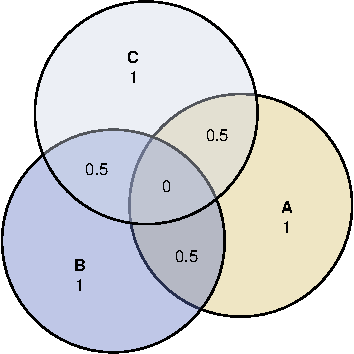
\includegraphics{thesis_files/figure-latex/unnamed-chunk-8-1.pdf}
\caption{\label{fig:unnamed-chunk-8}A plot with circles.}
\end{figure}

It is clear that this is not a good fit, which we can find out just by
looking at the plot. This is a good example of when ellipses come in
handy.

\begin{Shaded}
\begin{Highlighting}[]
\NormalTok{fit2 <-}\StringTok{ }\KeywordTok{euler}\NormalTok{(combo, }\DataTypeTok{shape =} \StringTok{"ellipse"}\NormalTok{)}
\NormalTok{fit2}
\end{Highlighting}
\end{Shaded}

\begin{verbatim}
##       original fitted residuals region_error
## A          1.0    1.0         0            0
## B          1.0    1.0         0            0
## C          1.0    1.0         0            0
## A&B        0.5    0.5         0            0
## A&C        0.5    0.5         0            0
## B&C        0.5    0.5         0            0
## A&B&C      0.0    0.0         0            0
## 
## diag_error:  0 
## stress:      0
\end{verbatim}

\begin{Shaded}
\begin{Highlighting}[]
\KeywordTok{plot}\NormalTok{(fit2, }\DataTypeTok{counts =} \OtherTok{TRUE}\NormalTok{)}
\end{Highlighting}
\end{Shaded}

\begin{figure}
\centering
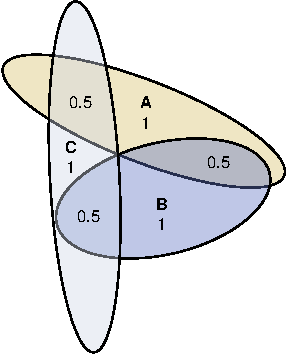
\includegraphics{thesis_files/figure-latex/unnamed-chunk-9-1.pdf}
\caption{\label{fig:unnamed-chunk-9}A plot with ellipses.}
\end{figure}

Much better.

\section{Plotting}\label{plotting}

Let's face it: euler diagrams are naught without visualization. Here,
\textbf{eulerr} interfaces the elegant Lattice graphics system {[}13{]}
to grant the user extensive control over the output, and allow for
facetted plots in case such a design was used in fitting the euler
configuration.

\subsection{Labelling}\label{labelling}

Most users will want to label their euler diagrams. One option is to
simply add a legend

\begin{Shaded}
\begin{Highlighting}[]
\KeywordTok{plot}\NormalTok{(}\KeywordTok{euler}\NormalTok{(}\KeywordTok{c}\NormalTok{(}\DataTypeTok{A =} \DecValTok{2}\NormalTok{, }\DataTypeTok{B =} \DecValTok{3}\NormalTok{, }\StringTok{"A&B"}\NormalTok{ =}\StringTok{ }\DecValTok{1}\NormalTok{)), }\DataTypeTok{auto.key =} \OtherTok{TRUE}\NormalTok{)}
\end{Highlighting}
\end{Shaded}

\begin{figure}
\centering
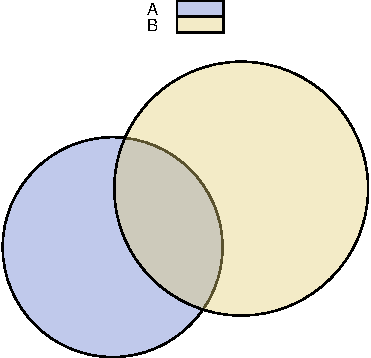
\includegraphics{thesis_files/figure-latex/unnamed-chunk-10-1.pdf}
\caption{\label{fig:unnamed-chunk-10}A simple plot.}
\end{figure}

but many will want to label their diagrams directly, perhaps with
counts.

\begin{Shaded}
\begin{Highlighting}[]
\KeywordTok{plot}\NormalTok{(}\KeywordTok{euler}\NormalTok{(}\KeywordTok{c}\NormalTok{(}\DataTypeTok{A =} \DecValTok{2}\NormalTok{, }\DataTypeTok{B =} \DecValTok{3}\NormalTok{, }\StringTok{"A&B"}\NormalTok{ =}\StringTok{ }\DecValTok{1}\NormalTok{)), }\DataTypeTok{counts =} \OtherTok{TRUE}\NormalTok{)}
\end{Highlighting}
\end{Shaded}

\begin{figure}
\centering
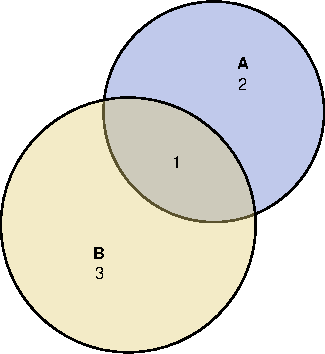
\includegraphics{thesis_files/figure-latex/unnamed-chunk-11-1.pdf}
\caption{\label{fig:unnamed-chunk-11}A plot with counts.}
\end{figure}

In this case, layout out the diagram becomes considerably more involved.
Finding a reasonable spot for the text inside the diagram only lends
itself to an easy solution if the shape of the intersection has a
center-of-gravity inside ellipse, in which case an average of some of
the points might suffice. This is often not the case, however, and we
need a better solution. Specifically, what we need is a method to find
the point inside the circle overlap for the counts and circle complement
to the intersection for our labels.

So far, we have not been able to derive at an analyitcal solution for
finding a good point, or for that matter a reliable way of finding
\emph{any} point that is in the required intersection or complement. As
is often the case, the next-best thing turns out to be a numerical one.
First, we locate a point that is inside the required region by spreading
points across one of the discs involed in the set combination. To spread
points uniformly, we use \emph{Vogel's method} {[}14,15{]} \[
\left( p_k = (\rho_k, \theta_k) = \left( r \sqrt{\frac{k}{n}},\, \pi (3 - \sqrt{5})(k - 1) \right) \right)_{k=1}^n,
\] which is actually based on the golden angle.

\begin{Shaded}
\begin{Highlighting}[]
\NormalTok{n <-}\StringTok{ }\DecValTok{500}
\NormalTok{seqn <-}\StringTok{ }\KeywordTok{seq}\NormalTok{(}\DecValTok{1}\NormalTok{, n, }\DecValTok{1}\NormalTok{)}
\NormalTok{theta <-}\StringTok{ }\NormalTok{seqn}\OperatorTok{*}\NormalTok{pi}\OperatorTok{*}\NormalTok{(}\DecValTok{3} \OperatorTok{-}\StringTok{ }\KeywordTok{sqrt}\NormalTok{(}\DecValTok{5}\NormalTok{))}
\NormalTok{rad <-}\StringTok{ }\KeywordTok{sqrt}\NormalTok{(seqn}\OperatorTok{/}\NormalTok{n)}
\NormalTok{x <-}\StringTok{ }\NormalTok{rad}\OperatorTok{*}\KeywordTok{cos}\NormalTok{(theta)}
\NormalTok{y <-}\StringTok{ }\NormalTok{rad}\OperatorTok{*}\KeywordTok{sin}\NormalTok{(theta)}

\KeywordTok{xyplot}\NormalTok{(x }\OperatorTok{~}\StringTok{ }\NormalTok{y, }\DataTypeTok{aspect =} \StringTok{"iso"}\NormalTok{, }\DataTypeTok{pch =} \DecValTok{20}\NormalTok{, }\DataTypeTok{xlab =} \StringTok{""}\NormalTok{, }\DataTypeTok{ylab =} \StringTok{""}\NormalTok{,}
       \DataTypeTok{col =} \DecValTok{1}\NormalTok{,}
       \DataTypeTok{par.settings =} \KeywordTok{list}\NormalTok{(}\DataTypeTok{axis.line =} \KeywordTok{list}\NormalTok{(}\DataTypeTok{col =} \StringTok{"transparent"}\NormalTok{)),}
       \DataTypeTok{scales =} \KeywordTok{list}\NormalTok{(}\DataTypeTok{draw =} \OtherTok{FALSE}\NormalTok{))}
\end{Highlighting}
\end{Shaded}

\begin{figure}
\centering
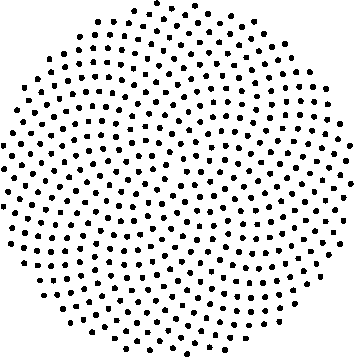
\includegraphics{thesis_files/figure-latex/unnamed-chunk-12-1.pdf}
\caption{\label{fig:unnamed-chunk-12}Spreading points on a disc with Vogel's
method.}
\end{figure}

After this, we scale, translate, and rotate the points so that they fit
the desired ellipse.

After we've spread our points throughout the ellipse and found one that
matches our desired combination of ellipses/sets, we then proceed to
optimize its position numerically. For this, we use version of the
\emph{Nelder--Mead Method} {[}16{]} which we've translated from Matlab
code by {[}17{]} and customized for \textbf{eulerr} (in particular to
make sure that the simplex does not escape the intersection boundaries
since we for this problem \emph{want} the local minimum).

\subsection{Coloring}\label{coloring}

Per default, the ellipses are filled with colors. The default option is
to use an adaptive scheme in which colors are chosen to provide a
balance between dinstinctiveness, beauty, and consideration for the
color deficient. The color palette has been generated from
\href{https://CRAN.R-project.org/package=qualpalr}{qualpalr} (developed
by the author), which automatically generates qualitative color palettes
based on a model of color perception.

\section*{References}\label{references}
\addcontentsline{toc}{section}{References}

\hypertarget{refs}{}
\hypertarget{ref-euler_1802}{}
1. Leonhard Euler. Letters of Euler to a German Princess, on Different
Subjects in Physics and Philosophy {[}Internet{]}. Murray; Highley; 1802
{[}cited 2017 Aug 14{]}. Available from:
\url{http://archive.org/details/letterseulertoa00eulegoog}

\hypertarget{ref-swinton_2011}{}
2. Swinton J. Vennerable: Venn and Euler area-proportional diagrams
{[}Internet{]}. Available from:
\url{https://github.com/js229/Vennerable}

\hypertarget{ref-micallef_2014}{}
3. Micallef L, Rodgers P. eulerAPE: Drawing Area-Proportional 3-Venn
Diagrams Using Ellipses. PLOS ONE. 201417ADJul;9(7):e101717.

\hypertarget{ref-wilkinson_2012}{}
4. Wilkinson L. Exact and Approximate Area-Proportional Circular Venn
and Euler Diagrams. IEEE Transactions on Visualization and Computer
Graphics. 2012 Feb;18(2):321--31.

\hypertarget{ref-kestler_2008}{}
5. Kestler HA, Müller A, Kraus JM, Buchholz M, Gress TM, Liu H, et al.
VennMaster: Area-proportional Euler diagrams for functional GO analysis
of microarrays. BMC Bioinformatics {[}Internet{]}. 2008 Jan {[}cited
2017 Aug 6{]};9:67. Available from:
\url{https://doi.org/10.1186/1471-2105-9-67}

\hypertarget{ref-schnabel_1985}{}
6. Schnabel RB, Koonatz JE, Weiss BE. A Modular System of Algorithms for
Unconstrained Minimization. ACM Trans Math Softw {[}Internet{]}. 1985
Dec {[}cited 2017 Aug 6{]};11(4):419--40. Available from:
\url{http://doi.acm.org/10.1145/6187.6192}

\hypertarget{ref-richter-gebert_2011}{}
7. Richter-Gebert J. Perspectives on Projective Geometry: A Guided Tour
Through Real and Complex Geometry. 1st ed. Berlin, Germany: Springer;
2011.

\hypertarget{ref-huber_2014}{}
8. Huber E. RConics: Computations on Conics {[}Internet{]}. 2014.
Available from: \url{https://CRAN.R-project.org/package=RConics}

\hypertarget{ref-eberly_area_2016}{}
9. Eberly D. The Area of Intersecting Ellipses {[}Internet{]}. Geometric
Tools. 2016 {[}cited 2017 Aug 7{]}. Available from:
\url{https://www.geometrictools.com/Documentation/AreaIntersectingEllipses.pdf}

\hypertarget{ref-eddelbuettel_2011}{}
10. Eddelbuettel D, François R. Rcpp: Seamless R and C++ integration.
Journal of Statistical Software {[}Internet{]}. 2011;40(8):1--18.
Available from: \url{http://www.jstatsoft.org/v40/i08/}

\hypertarget{ref-eddelbuettel_2014}{}
11. Eddelbuettel D, Sanderson C. RcppArmadillo: Accelerating r with
high-performance c++ linear algebra. Computational Statistics and Data
Analysis {[}Internet{]}. 2014 March;71:1054--63. Available from:
\url{http://dx.doi.org/10.1016/j.csda.2013.02.005}

\hypertarget{ref-jylanki_2010}{}
12. Jylänki J. A Thousand Ways to Pack the Bin - A Practical Approach to
Two-Dimensional Rectangle Bin Packing {[}Internet{]}. 2010 {[}cited 2017
Aug 7{]}. Available from:
\url{http://clb.demon.fi/files/RectangleBinPack.pdf}

\hypertarget{ref-sarkar_2008}{}
13. Sarkar D. Lattice: Multivariate Data Visualization with R
{[}Internet{]}. New York, USA: Springer; 2008. (Use R!). Available from:
\url{http://www.springer.com/us/book/9780387759685}

\hypertarget{ref-arthur_2015}{}
14. Arthur MK. Point Picking and Distributing on the Disc and Sphere
{[}Internet{]}. Abedeen, USA: US Army Research Laboratory, Weapons;
Materials Research Directorate; 2015 Jul p. 58. Report No.: ARL-TR-7333.
Available from: \url{www.dtic.mil/get-tr-doc/pdf?AD=ADA626479}

\hypertarget{ref-vogel_1979}{}
15. Vogel H. A better way to construct the sunflower head. Mathematical
Biosciences. 1979;44(3-4):179--89.

\hypertarget{ref-nelder_1965}{}
16. Nelder JA, Mead R. A Simplex Method for Function Minimization. The
Computer Journal {[}Internet{]}. 1965 Jan;7(4):308--13. Available from:
\url{https://academic.oup.com/comjnl/article/7/4/308/354237/A-Simplex-Method-for-Function-Minimization}

\hypertarget{ref-kelley_1999}{}
17. Kelley CT. Iterative Methods for Optimization. 1 edition.
Philadelphia, USA: Society for Industrial; Applied Mathematics; 1999.
(Frontiers in applied mathematics).


\end{document}
